\documentclass[a4paper,12pt,oneside,fleqn]{article}
\usepackage[latin1]{inputenc}
\usepackage[T1]{fontenc}
\usepackage[finnish, english]{babel}
\usepackage{times}
\usepackage[pdftex]{graphicx}
\usepackage[left=35mm,right=20mm,top=20mm,bottom=25mm]{geometry}
\usepackage{setspace}
\usepackage{sectsty}
\usepackage{fancyhdr}
\usepackage{icomma}
\usepackage{amssymb,amsmath}
\usepackage[titles]{tocloft}
\usepackage{ccaption}
\usepackage{natbib}
\usepackage{colortbl}
\usepackage{listings}
\usepackage{hyperref}
\usepackage[none]{hyphenat}
\sloppy

\hypersetup{
  pdfproducer={pdflatex},
  colorlinks=true,
  linkcolor=red,
  citecolor=green,
  filecolor=magenta,
  urlcolor=blue
}

\graphicspath{{figures/}}

\setlength{\headheight}{10mm}
\pagestyle{fancy}
\renewcommand{\headrulewidth}{0pt}
\renewcommand{\footrulewidth}{0pt}
\singlespacing
\newenvironment{equation_text}[0]
{\begin{list}{}{\setlength{\leftmargin}{25mm}}}
{\end{list}}

\newcommand{\researchname}[0]{Final report}

\newcommand{\flabel}[1]{\label{fig:#1}}
\newcommand{\tlabel}[1]{\label{tab:#1}}
\newcommand{\elabel}[1]{\label{eq:#1}}
\newcommand{\slabel}[1]{\label{sec:#1}}

\newcommand{\fref}[1]{Figure~\ref{fig:#1}}
\newcommand{\tref}[1]{Table~\ref{tab:#1}}
\newcommand{\eref}[1]{Equation~\ref{eq:#1}}
\newcommand{\sref}[1]{Section~\ref{sec:#1}}

\newcommand{\tcaption}[1]{\caption{#1}\vspace{3mm}}

\newenvironment{enu}
{\begin{enumerate}
	\setlength{\topsep}{0pt}
  \setlength{\itemsep}{0pt}
  \setlength{\partopsep}{0pt}
  \setlength{\parskip}{0pt}
  \setlength{\parsep}{0pt}}
{\end{enumerate}}

\newenvironment{ite}
{\begin{itemize}
	\setlength{\topsep}{0pt}
  \setlength{\itemsep}{0pt}
  \setlength{\partopsep}{0pt}
  \setlength{\parskip}{0pt}
  \setlength{\parsep}{0pt}}
{\end{itemize}}

\renewcommand{\cftsecfont}{\normalfont}
\renewcommand{\cftsecpagefont}{\normalfont}
\renewcommand{\cftsecleader}{\cftdotfill{\cftdotsep}}
\setcounter{tocdepth}{3}
\setlength{\parskip}{0mm}
\setlength{\parindent}{0mm}
\setlength{\mathindent}{15mm}

\sectionfont{\fontfamily{phv}\fontseries{b}\fontsize{16pt}{18pt}\selectfont\uppercase}
\subsectionfont{\fontfamily{phv}\fontseries{b}\fontsize{14pt}{16pt}\selectfont}
\subsubsectionfont{\fontfamily{phv}\fontseries{m}\fontsize{12pt}{16pt}\selectfont}

\captiondelim{. }
\captionstyle{\raggedright}
\precaption{\hspace{5mm}}
\captiontitlefont{\fontfamily{phv}\fontshape{it}\fontsize{11pt}{12pt}\selectfont}
\bibpunct{/}{/}{,}{n}{}{,}

\definecolor{lightgrey}{rgb}{.8,.8,.8}
\definecolor{lightlightgrey}{rgb}{.9,.9,.9}
\definecolor{darkgrey}{rgb}{.5,.5,.5}
\definecolor{darkdarkgrey}{rgb}{.4,.4,.4}

\begin{document}

\renewcommand{\figurename}{\fontfamily{phv}\fontseries{b}\fontsize{11pt}{12pt}\selectfont Figure}
\renewcommand{\tablename}{\fontfamily{phv}\fontseries{b}\fontsize{11pt}{12pt}\selectfont Table}

% TITLE PAGE
\thispagestyle{empty}
\addtolength{\hoffset}{-5mm}
\begin{flushleft}
{\fontfamily{phv}\selectfont\textbf{EINDHOVEN UNIVERSITY OF TECHNOLOGY}} \\
{\fontfamily{phv}\selectfont\textbf{Department of Mathematics and Computer Science}} \\
{\fontfamily{phv}\selectfont\textbf{Department of Computer Science}} \\
{\fontfamily{phv}\selectfont\textbf{2ID35 Database Technology}} \\
{\fontfamily{phv}\selectfont\textbf{Project}} \\
\end{flushleft}

\vfill

\begin{center}
{\fontfamily{phv}\selectfont\textbf{\researchname}} \\
%{\fontfamily{phv}\selectfont Supervisor: Title Supervisor name} \\
\end{center}

\vfill

\begin{flushright}
\begin{tabular}{l}
{\fontfamily{phv}\selectfont In Eindhoven} \\
{\fontfamily{phv}\selectfont 12.06.2010} \\
{\fontfamily{phv}\selectfont Puputti Kimmo (0735552), Geert Kemps (0514520)} \\
%{\fontfamily{phv}\selectfont student number} \\
{\fontfamily{phv}\selectfont k.p.puputti@student.tue.nl, g.c.m.kemps.1@student.tue.nl }
\end{tabular}
\end{flushright}
\clearpage

% SECTIONS
\pagestyle{fancy}
\fancyhf{}
\rhead{\thepage}
\setcounter{page}{1}
\setstretch{1.1}

\section{Motivation}
With the increasing amount of web services available, privacy becomes
a popular topic. An indication of how valuable personal data can be is
the revenue made by Google, who can reach billion individuals while
collecting, for example, their search queries. On the other hand,
people benefit from services like Google. They can search the web and
communicate with friends and family.\\

Since these services are often free in terms of money, it does not
mean the customer doesn't has to pay a price. They pay the price in
terms of privacy. According to \cite{Jiang}, transparency is one of
the key foundations of privacy. The user should know how his or her
data is being treated, stored and to whom it will be disclosed. Then
the user can estimate if the 'price' he pays is worth the service.\\

Also, it is not that customers do not trust service providers, data
can always be subject to third party attacks, government regulation
etc. No service has been proven 100\% secure and still useable. Some
examples are the servers of the Pentagon \cite{Pentagon} and FBI
\cite{FBI}. \\

This privacy violation will only increase with the growth of data
collection. A way to reduce the privacy risk is to limit the data
retention. Limited retention is a widely accepted privacy
principle. It means that the data should not be stored longer than
necessary to fulfill its purpose.\cite{hippocratic-dbs} However this
limited retention is difficult to put in practise. How can we
determine these retention periods? It might be a better idea to find a
mechanism to balance privacy and usability, as is proposed in our
paper. \cite{Heerde}\\

Other proposals include making the data donors themselves responsible
for protecting their data.\cite{Aggarwal} \cite{W3C} This is a good
solution against server attacks, but leads to less accessability for
the service providers and high communication costs. In addition
security measures as data encryption, firewalls and intrusion
detection can be used. But they can only make attacks harder, not
prevent them. Finally anonymization may be a solution to prevent
disclosure of privacy sensitive data. Major companies, such as Google
\cite{Fleischer}, have already started using anonymization to improve
the privacy of their users. Data degradation does not aim at
generalizing identities, but can still be compared with respect to
generalization techniques. But, correctly anonymizing can be a hard
problem. AOL published and anonymized the IP addresses from which
queries were issued, but was proven not enough when hackers inferred
privacy sensitive facts. \cite{Hillyard} Data degradation will not be
vulnerable to this, because the facts themselves will be degraded.



\section{Research problems in the article}

Normally companies have some fixed time that information is saved, and
after the data is old enough, it is removed completely. This presents
many problems, since the data is valuable to the providers, but the
removal of data is important for respecting the privacy of the
users.\\

With the service providers' and users' needs being the opposite of
each other, a better way to save and remove data is needed. Van Heerde
et al. propose a way to degrade the data over time, so that not all
information is kept over time, but some parts of it is removed. This
tries to be a compromise between the needs of the providers and the
needs of the users.\\

By keeping some data around longer, the service providers can still
use the valuable data for their needs, but the privacy of the users is
better than in the case where all data is kept. With the degraded
data, the information about the users is not so accurate anymore, and
possible data breaches don't affect the users that much anymore.\\

Van Heerde et al. present a framework for degrading the data over
time. It tries to optimize the common interest of the service
providers and the users by balancing privacy and data usability. The
framework allows to compute the interest of the service providers and
the interest of the users separately, and offers a way to combine
these to a common interest.

\section{Results in the article}

The framework for data degradation described in the article by Van
Heerde et al. used two functions for computing the common interest  of
the service providers and the users. First function computes the worth
of storing the data for the service provider, and the second one
computes the risk for involved for storing the data.\\

With the defined functions, Van Heerde et al. were able to find the
optimal retention period $\delta_{opt}$ so that the common interest
$CI(\delta_{opt})$ of the both parties was respected.\\

The common interest of the two parties depends on many
factors. Sometimes the decrease of worth is higher than the increase
in privacy. Van Heerde et al. showed that progressively degrading the
data is useful in the cases they presented.\\

The following functions were derived:

\[
    totworth(\vec\delta) = c \times \sum_{l=0}^{n-1}
    \sum_{a=\delta_l}^{\delta_{l+1} + 1} wt_l(a)
\]
Where $c$ is a constant. $a,\delta$ range over age (time interval) and
$l$ is the level of accuracy.
\[
    risk(\vec\delta) = c \times \sum_{l=0}^{n-1} r_l \times
    (\delta_{l+1} - \delta_l)
\]
Where $r_l$ is the weight of the risk of storing a datum in level
$L_l$, with $r_l$ such that $1 = r_0 \geq r_1 \geq \ldots \geq
r_{n-1}$.
\[
    priv(\vec\delta) = \frac{1}{(s + risk(\vec\delta))}
\]
\[
    CI(\vec\delta) = totworth(\vec\delta) \times priv(\vec\delta)
\]

The above functions were applied to $n = 4$, a monotonic descending
function $wt_l(a)$ and some fixed values for $w_i$ and $r_i$. A script
found the $\vec\delta$ for which common interest is maximal.  The
following conclusions were drawn from the results:

\begin{itemize}
    \item Common interest is higher when progressively degradation ($n
      > 1$) the data than with limited retention of accurate data
      ($n=1$).

    \item With $n > 1, \delta_1$ is smaller than the single $\delta$
      with $n =1$. So it makes sense to degrade the data earlier to
      achieve a higher common interest.

    \item When $n = 4$, it turns out that $\delta_3 =
      \delta_4$. Meaning it is not possible to achieve an higher
      common interest with more than 3 degradation steps.
\end{itemize}

\section{Verifying the claims}

%% For evaluating the results of the article, we are going to use the
%% proposed methods for data degradation for a part of the query log data
%% set released by AOL a few years ago (
%% http://techcrunch.com/2006/08/06/aol-proudly-releases-massive-amounts-of-user-search-data/
%% ).\\

%% The query log contains 36 million records with five fields: id of the
%% user, query string, time of the query, ranking of the clicked link,
%% and the clicked link itself. The last two fields can be empty.\\

%% The data set is analyzed using Python programming language. If some
%% plots are needed for visualizing the results, Matplotlib Python
%% plotting library ( http://matplotlib.sourceforge.net/ ) is used.\\

%% We will provide means for calculating the worth of the data and the
%% risk of the data automatically. We will then find the optimal common
%% interest for the data and try to degrade it using the functions
%% created. Then we will compare the results of the different levels of
%% degradation to get comparable results.

\subsection{Validating results of the article}

We created a script \texttt{validate.py} (see Appendix A) that counts
the CI, totworth, priv, and risk numbers for the data used in the
article. By running the script we get the following output:

\begin{verbatim}
$python validate.py
CI(d): 1.37136663791
totworth(d): 61.7114987058
priv(d): 0.0222222222222
risk(d): 27.0
\end{verbatim}

which corresponds to the values obtained in the article.

\subsection{Extending the article to a real world data set}

We used a part of the AOL query log data
set\footnote{\href{http://techcrunch.com/2006/08/06/aol-proudly-releases-massive-amounts-of-user-search-data/}{http://techcrunch.com/2006/08/06/aol-proudly-releases-massive-amounts-of-user-search-data/}}. We
extracted the log data for one single user that had the most queries
made within the period and that was not an automatically querying
bot. There are 3646 records with the earliest made on March 1 2006 and
the latest made on May 31 2006.

In the article, Van Heerde et. al made a simplifying assumption that
the insert rate of data is constant over time. This does not reflect
reality, and we tried to extend the techniques to data that has a
random insert rate.

We created a script \texttt{degrade.py} that can be run with the
command:

\begin{verbatim}
python degrade.py graphs
\end{verbatim}

that creates several figures to the `output' directory. Some of the
created figures are shown in \fref{ages}, \fref{worths},
\fref{privacies}, \fref{totworths}, and \fref{cinterests}.

\begin{figure}[h]
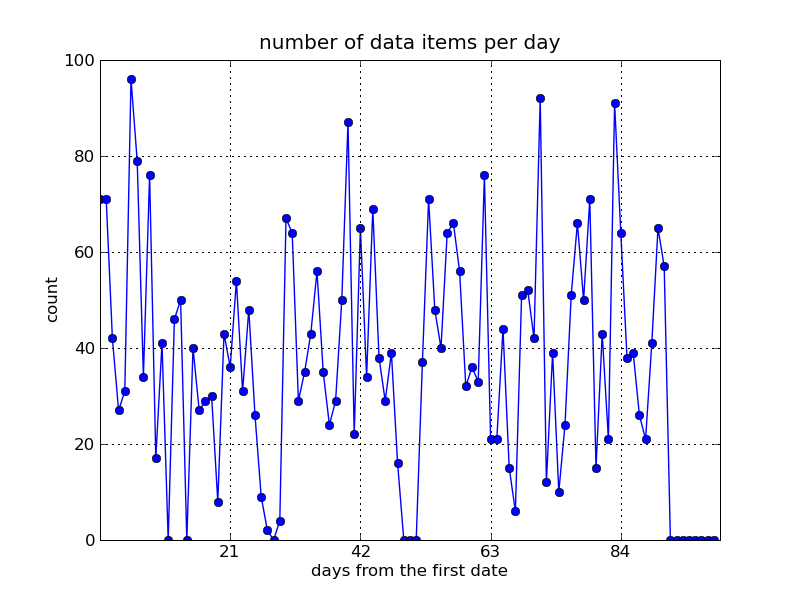
\includegraphics[width=\linewidth]{img/ages.png}
\caption{Data items inserted per day.}
\flabel{ages}
\end{figure}

\begin{figure}[h]
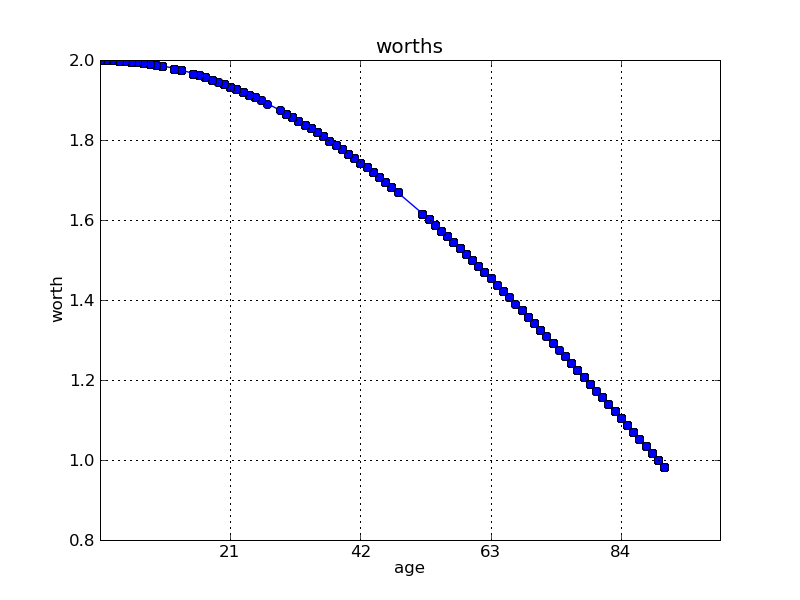
\includegraphics[width=\linewidth]{img/worths.png}
\caption{Worths of data items.}
\flabel{worths}
\end{figure}

\begin{figure}[h]
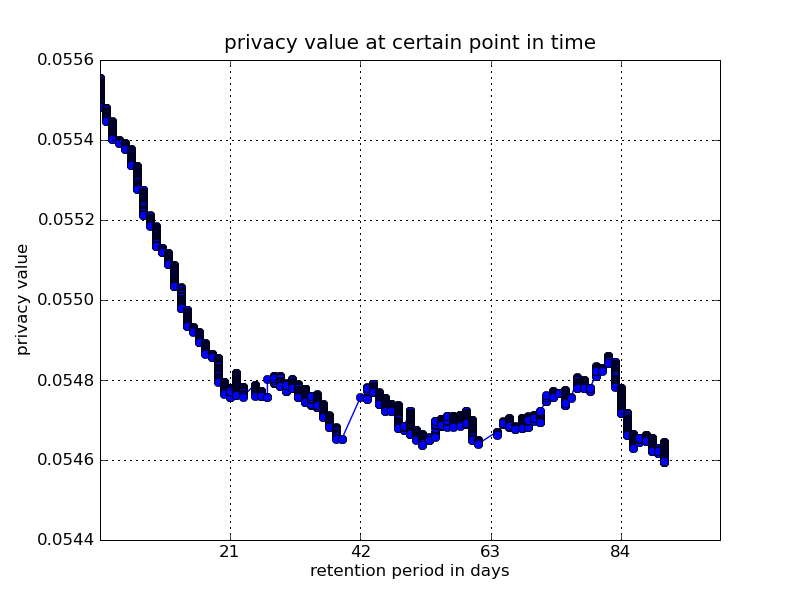
\includegraphics[width=\linewidth]{img/privacies.png}
\caption{Privacy of the data items.}
\flabel{privacies}
\end{figure}

\begin{figure}[h]
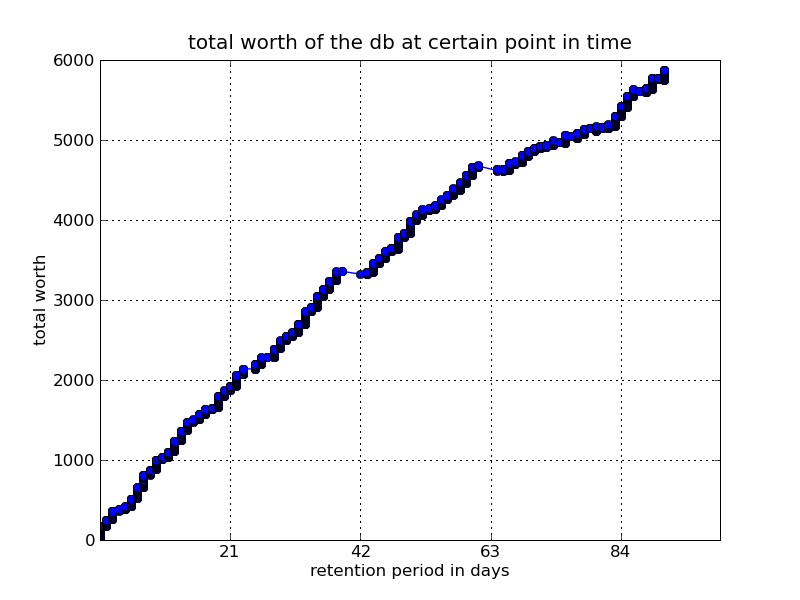
\includegraphics[width=\linewidth]{img/tot_worths.png}
\caption{Total worth of the data items.}
\flabel{totworths}
\end{figure}

\begin{figure}[h]
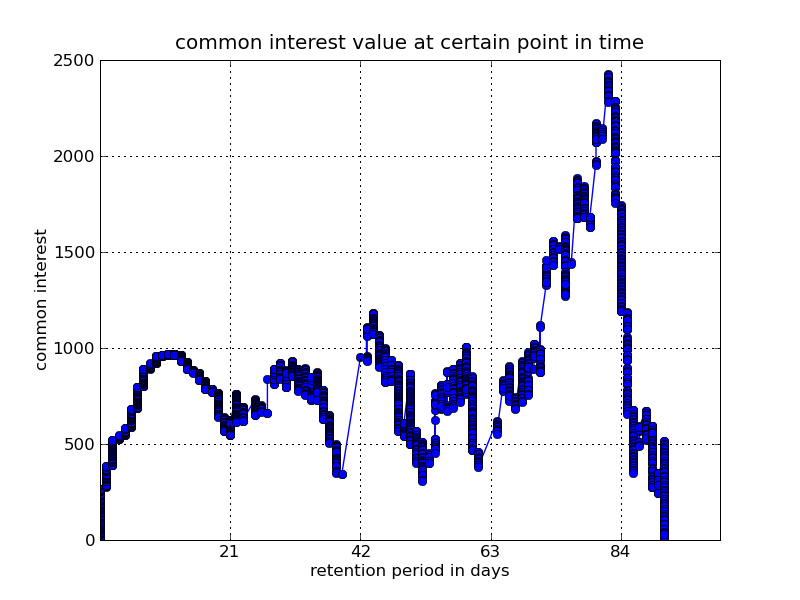
\includegraphics[width=\linewidth]{img/common_interests.png}
\caption{Common interest for the data items.}
\flabel{cinterests}
\end{figure}

\clearpage
\section{Results}

As can be seen from \fref{cinterests}, there is something weird
happening in the common interest values. There should be a single
point where the common interest value is higher than in points before
or after it. However, our graph has several local maximums and a large
spike at the end of it. We expect this to be a mistake in applying the
techniques of a constant insert rate data to a randomly inserted
data. It is also possible that there is something wrong in our
calculations. However, \fref{privacies} and \fref{totworths} indicate
that the graphs are of the right shape compared to the ones in the
article. Therefore, mistakes in our methodologies might have happened
in combining the privacy and total worth values to calculate the
common interest values.\\

Apart from our inability to extend the results to a randomly inserted
data, we still claim to believe that the methodologies of Van Heerde
et. al. are applicable to any kind of data set. The all-or-nothing
method should always be worse than data degradation, and both the
service providers and the users can make a compromise that benefits
both parties.

\clearpage
\nocite{*}
\bibliography{mybib}
\bibliographystyle{plain}

% Set code listing styles.
\lstset{
language=Python,
basicstyle=\footnotesize\ttfamily,
numbers=left,
numberstyle=\tiny,
numberstyle=\footnotesize,
showstringspaces=false
}

\clearpage
Appendix A: validate.py:
\lstinputlisting{../../src/validate.py}

\clearpage
Appendix B: degrade.py:
\lstinputlisting{../../src/degrade.py}

\end{document}
